\subsection{Wagasci modules}
The Wagasci modules are neutrino target detector consists of 16 scintillator tracking planes, where each plane is an array of 80 scintillator bars.
The total number of channels in one Wagasci module is 1280.
The 40 bars, called parallel scintillators, are placed perpendicularly to the beam, and the other 40 bars, called grid scintillators, are placed in parallel to the beam with grid structure in the tracking plane as shown in Fig. \ref{fig:3dgrid_wagascimod}.
Thanks to the 3 D grid-like structure of the scintillator bars, 
the Wagasci module has $4\pi$ angular acceptance for charged particles.
Thin plastic scintillator bars (3 mm in thickness, Figure \ref{fig:wagasci_scinti_geometry}) are used for the Wagasci modules
to reduce the mass ratio of scintillator bars to water,
because neutrino interactions in the scintillator bars are a background for the cross section measurements on H$_{2}$O.
The dimension of the each Wagasci module is 125cm $\times$ 125cm in the x and y directions
and 46cm along the beam direction as shown in \ref{fig:3dgrid_wagascimod}.

\begin{figure}[tbhp]
  \begin{center}
   \begin{subfigure}{0.48\textwidth}
     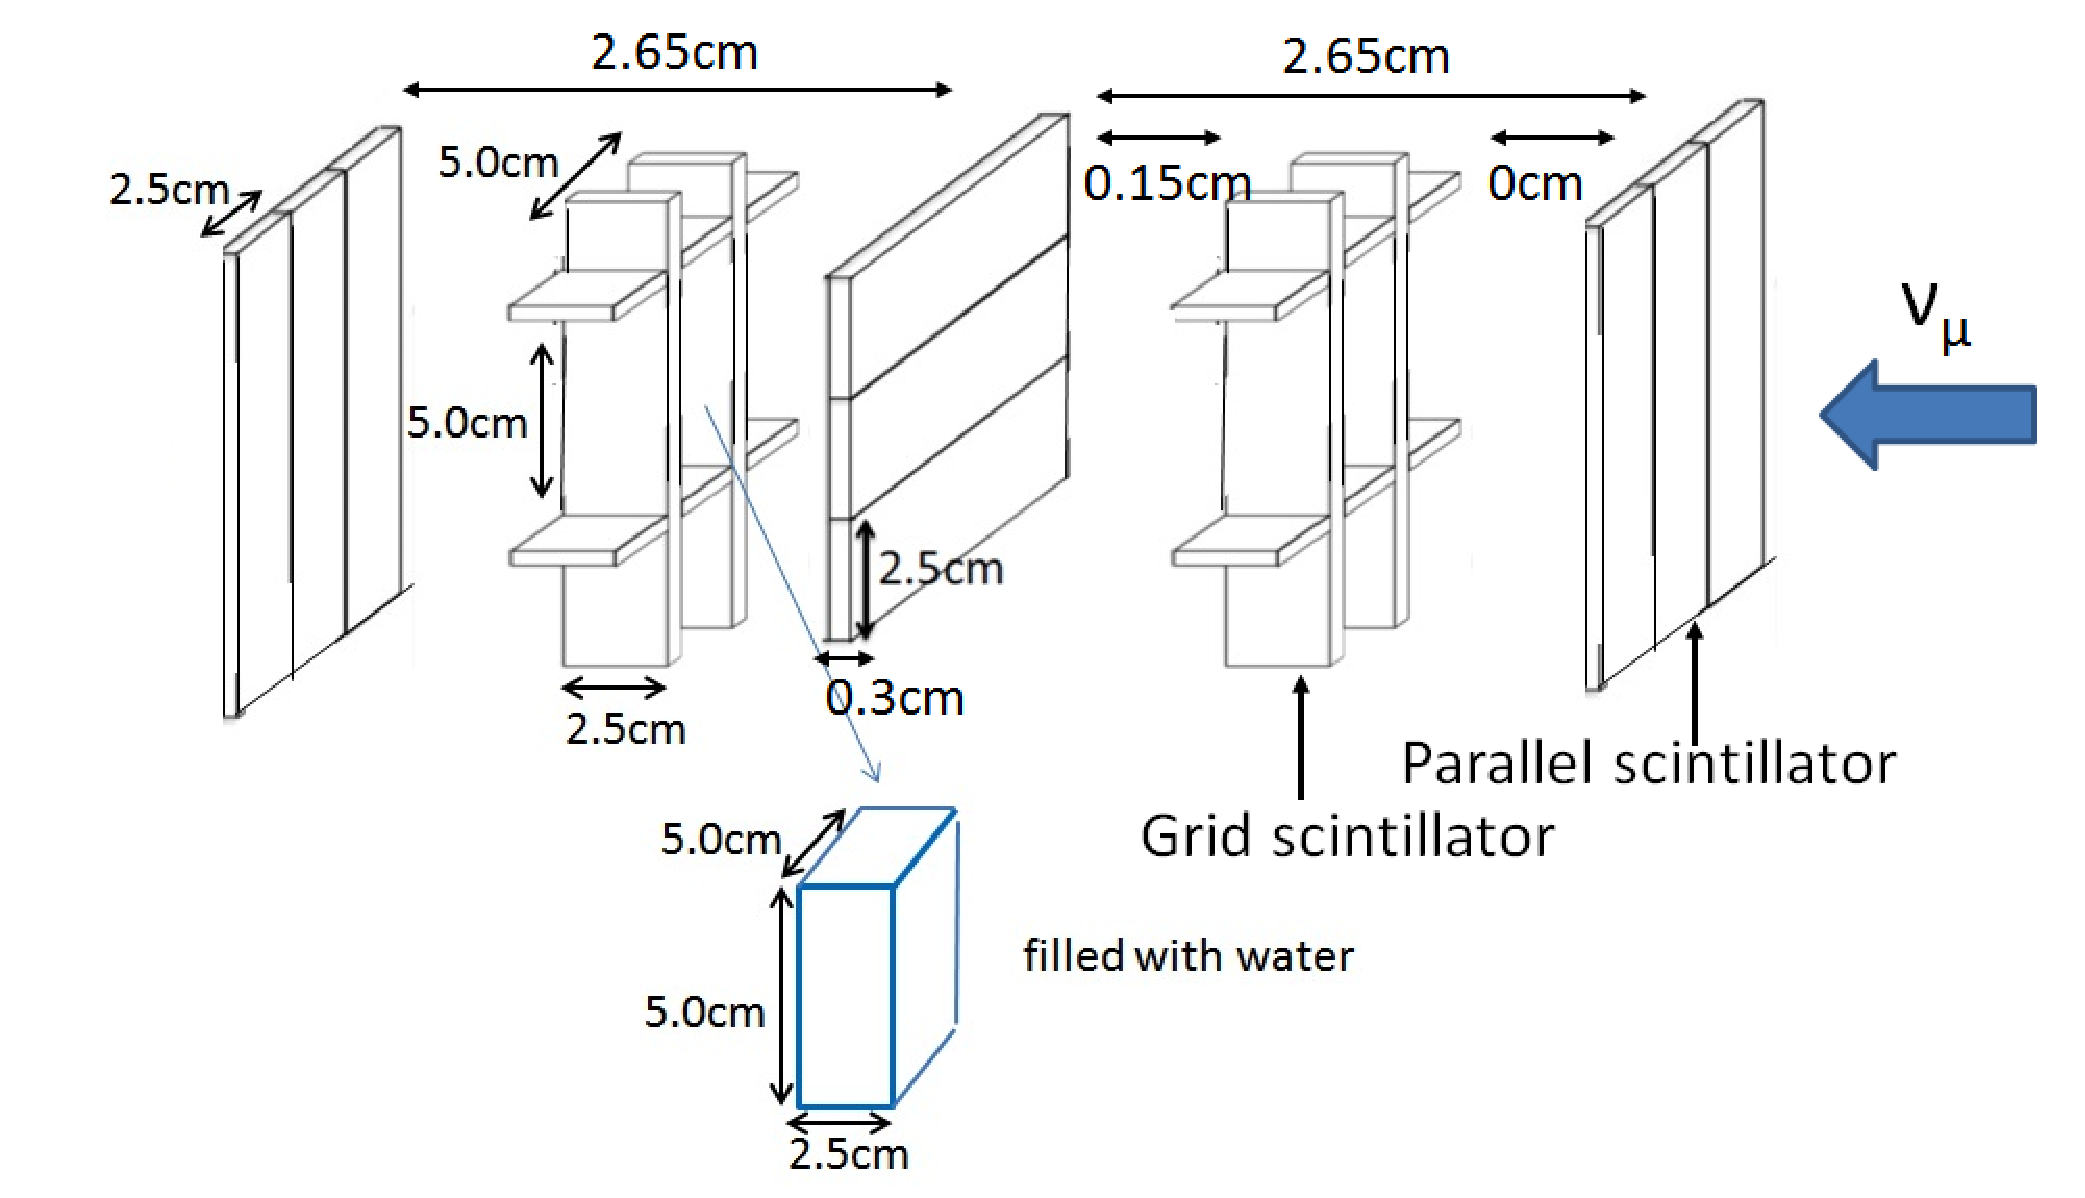
\includegraphics[width=\linewidth]{fig/3d_grid_structure.pdf}
    \end{subfigure}
  \begin{subfigure}{0.48\textwidth}
      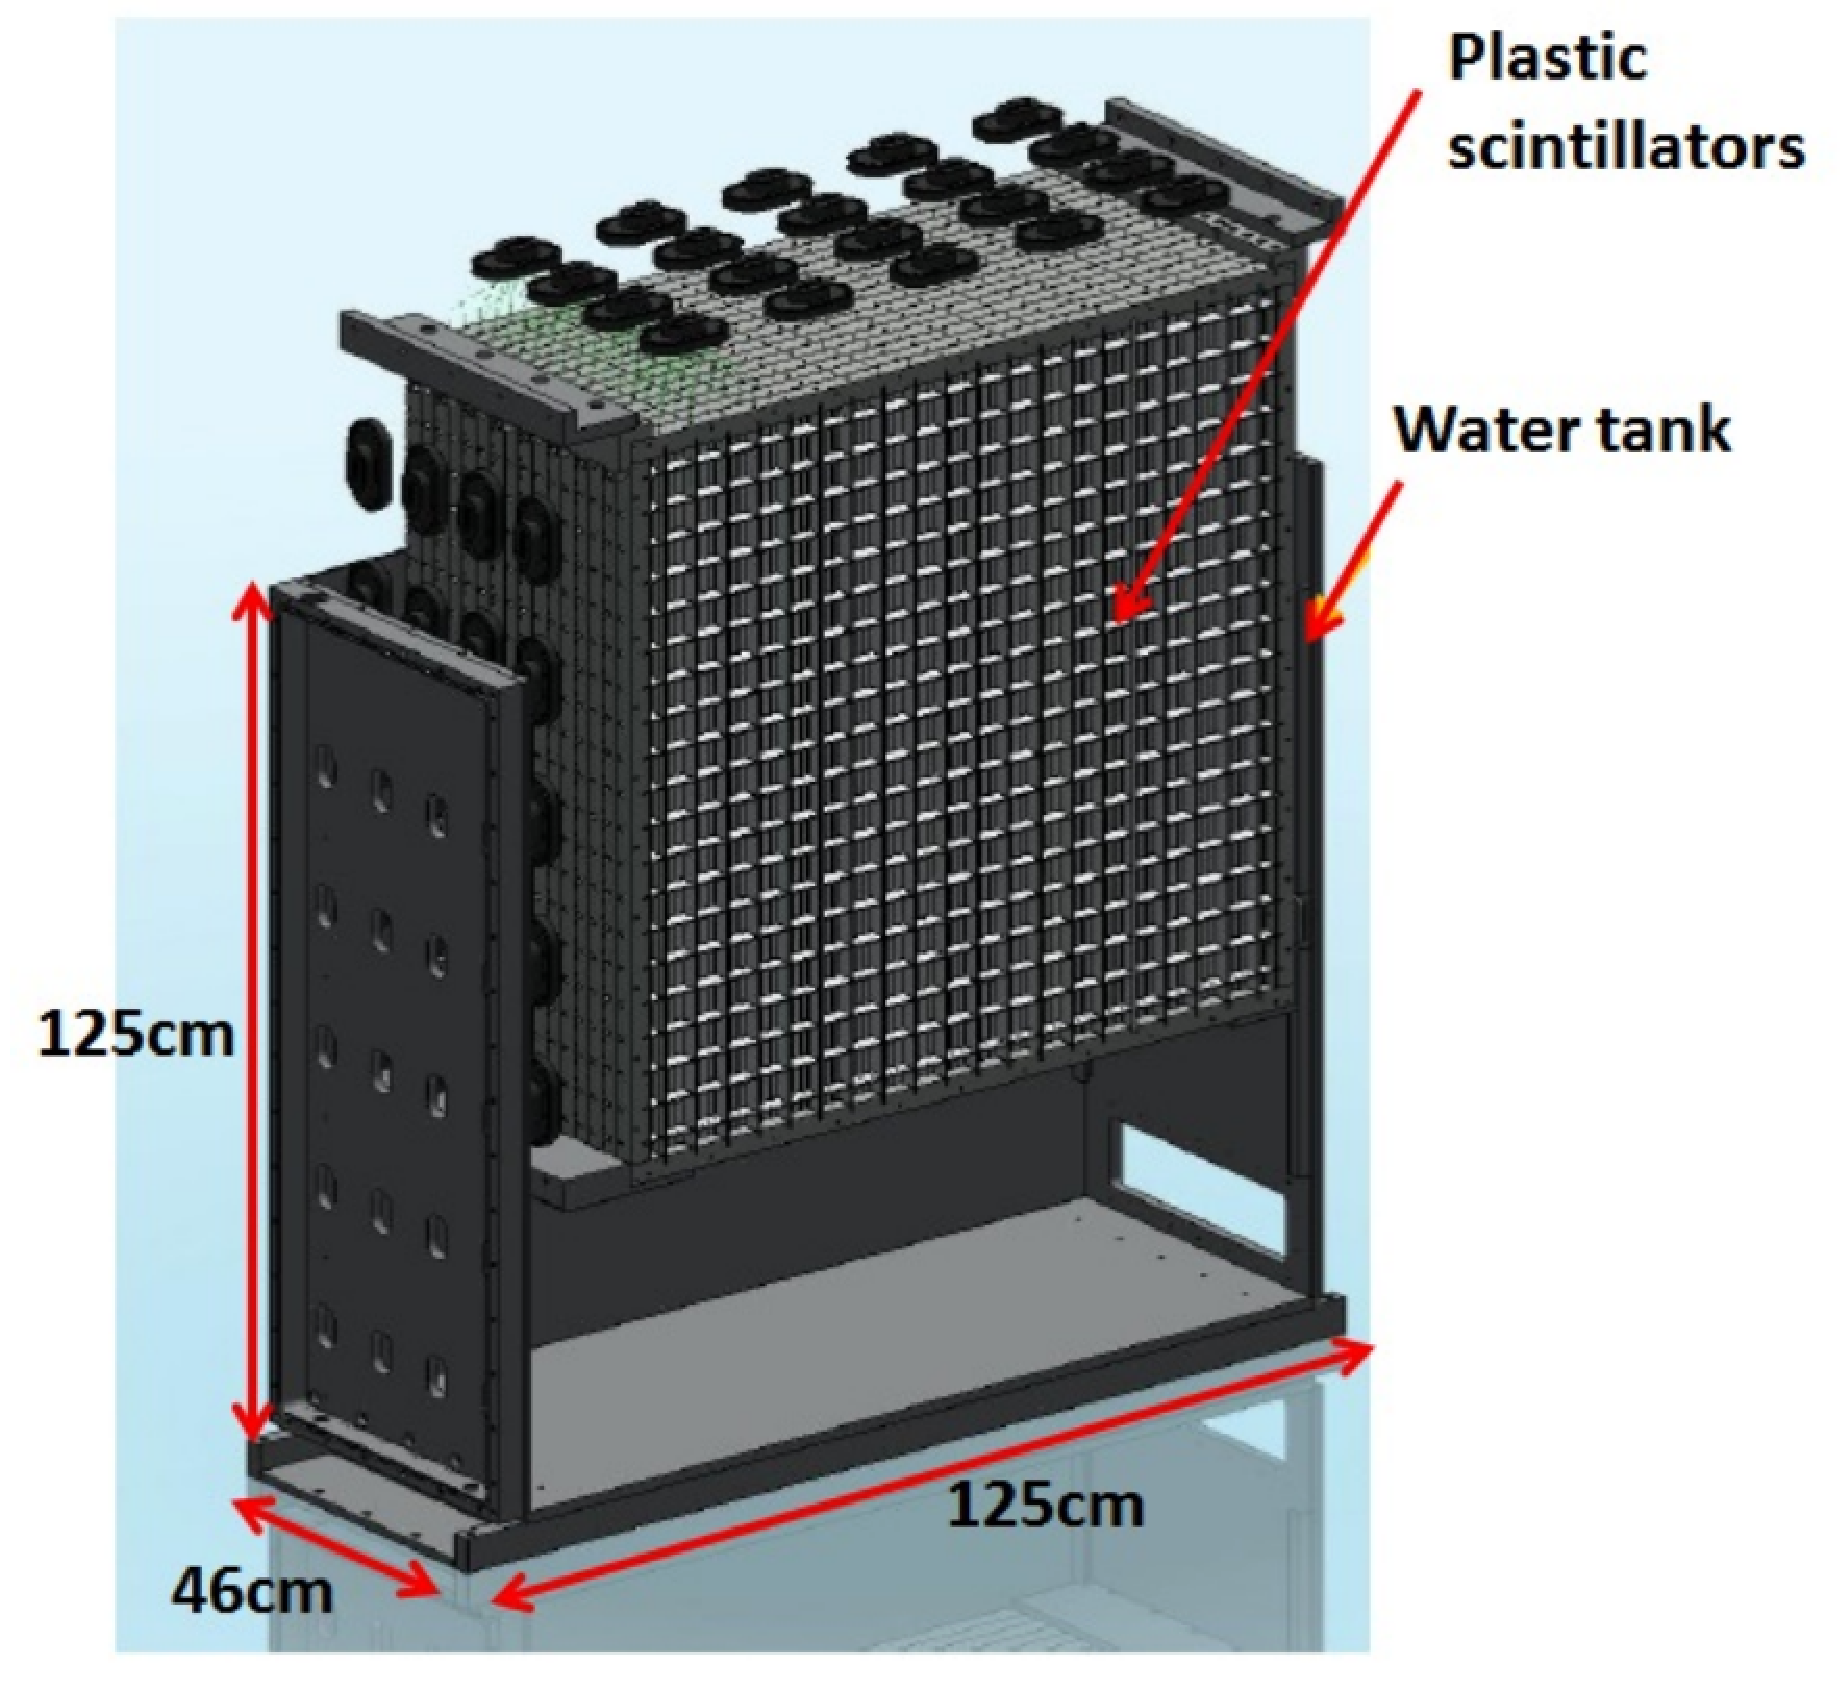
\includegraphics[width=\linewidth]{fig/wagasci_mod.pdf}
    \end{subfigure}    
    \end{center}
  \caption{Schematic views of 3D grid-like structure of plastic scintillator bars (left) and Wagasci module (right).}
\label{fig:3dgrid_wagascimod}
\end{figure}

\begin{figure}[tbh]
\begin{center}
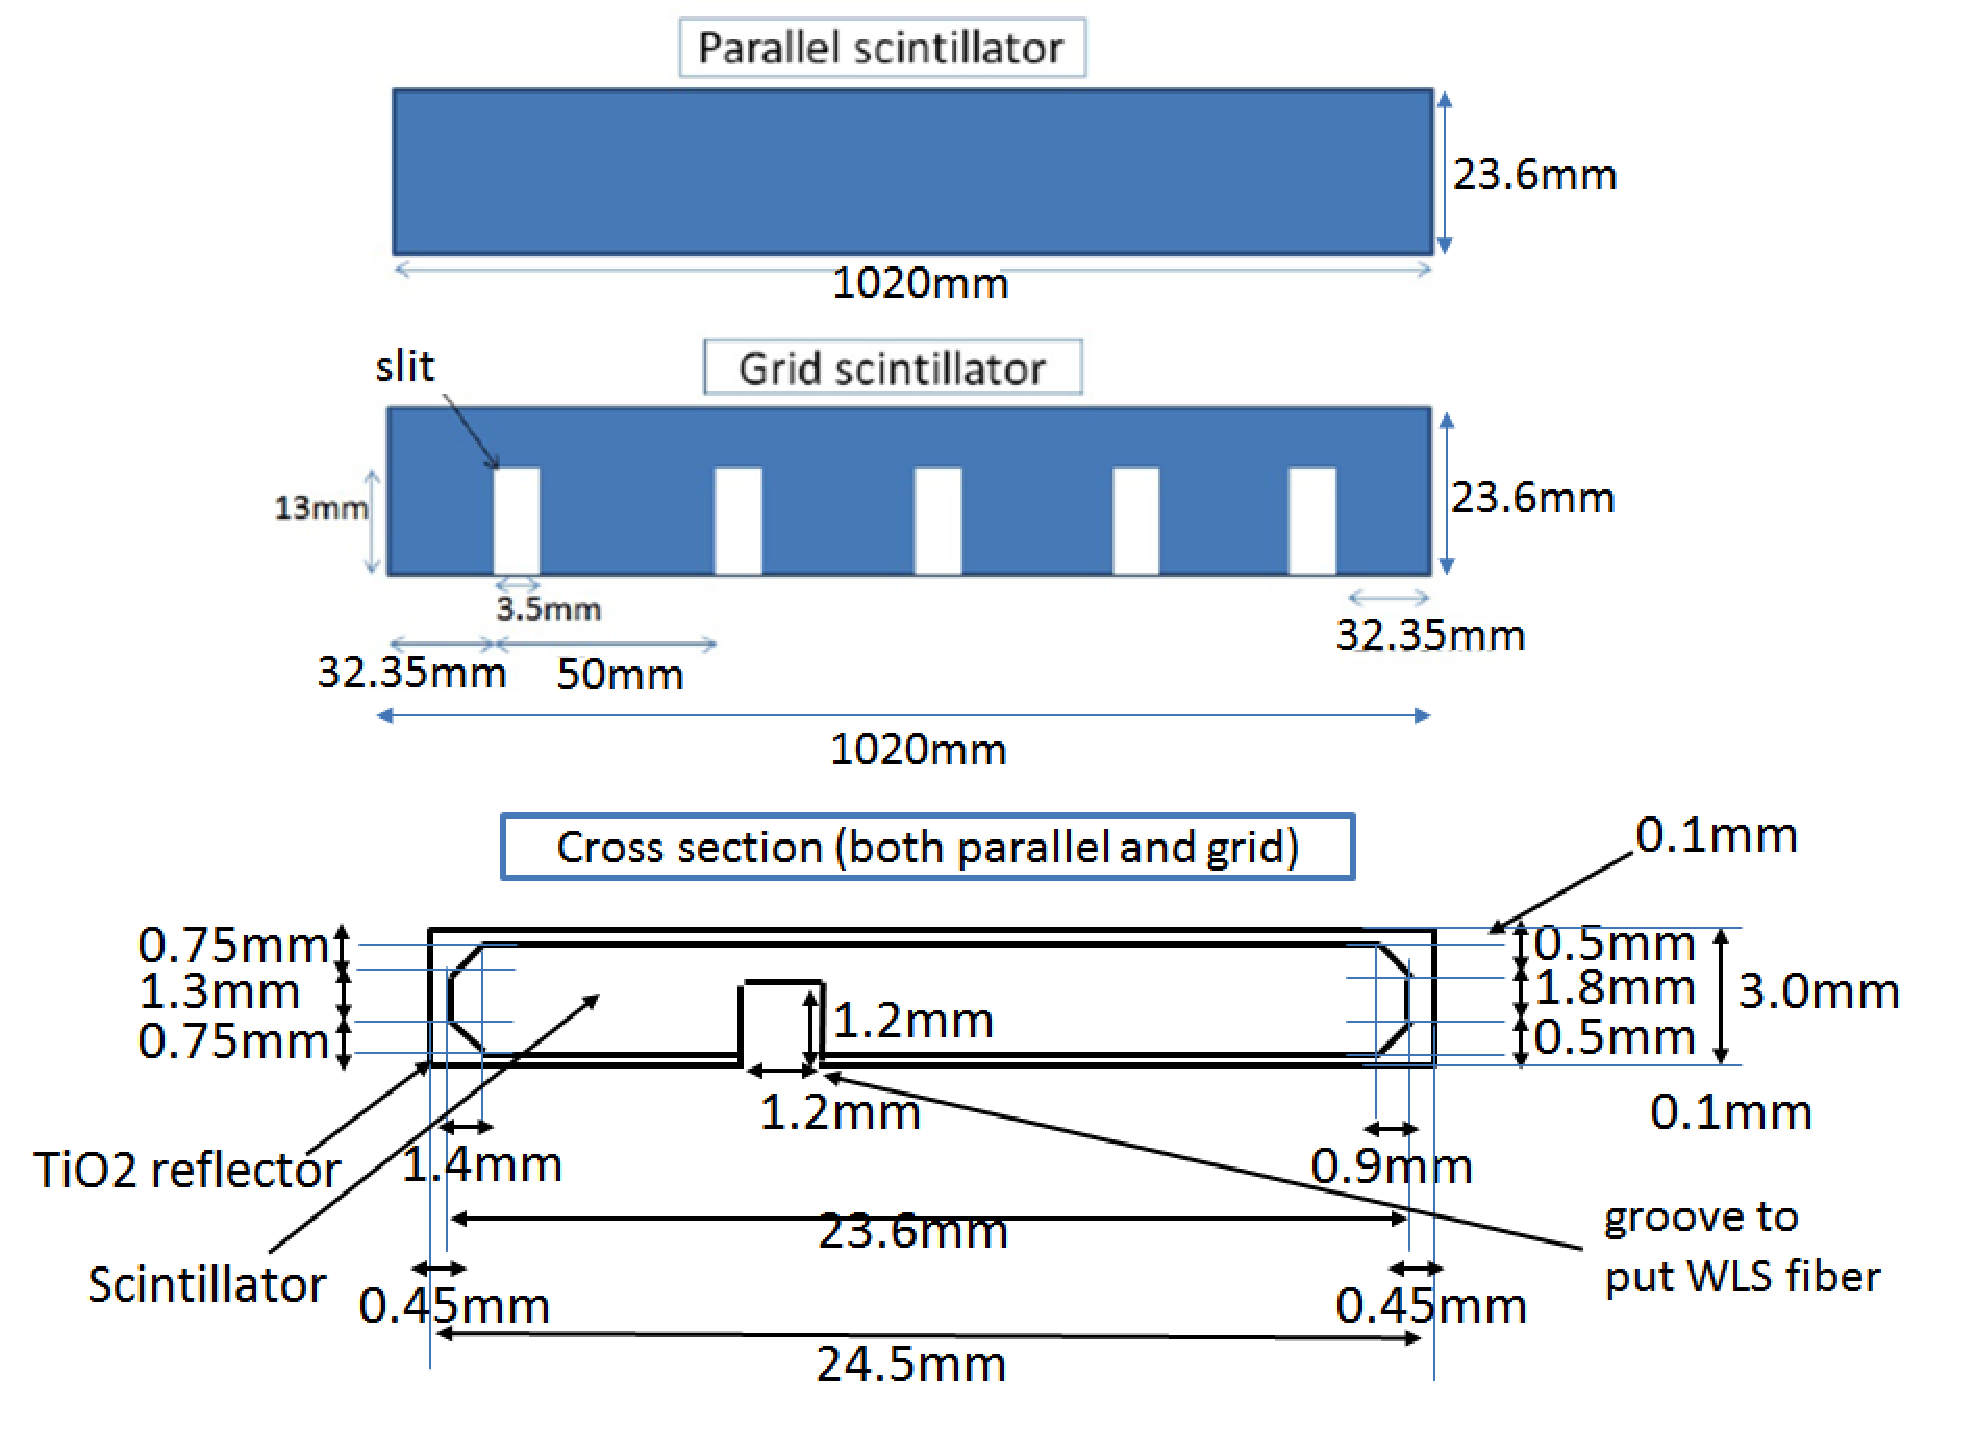
\includegraphics[width=0.8\linewidth]{fig/wagasci_scinti_geometry.pdf}
% 
\includegraphics[width=0.6\linewidth]{fig/tmp.pdf}
\end{center}
\caption{
Geometry of scintillators used for Wagasci modules.
}
\label{fig:wagasci_scinti_geometry}
\end{figure}


We will have two types of the Wagasci modules, a water-in module and a water-out module.
The water-in Wagasci module has water in spaces of the grid structure.
The total water mass serving as neutrino targets in the fiducial volume of the module is 188 kg,
and the mass ratio of scintillator bars to water is 80 \%.
The water-out Wagasci module doesn't have water inside the detector.
The total CH mass serving as neutrino target in the fiducial volume of the module is 47 kg,
and the mass fraction of scintillator bars is 100 \%.

